\documentclass[11pt]{article}
\usepackage[margin=1.0in]{geometry}
\addtolength{\topmargin}{0.25in}
\usepackage[document]{ragged2e}
\usepackage{graphicx}
\graphicspath{{../pictures/}}
\usepackage{float}
\usepackage{siunitx}


\begin{document}
	{\Huge\textbf{EEE381 Tech Memo}}\\
	\hfill \break
	\textbf{From:} Charles Noah Lutz\\
	\textbf{Partner:} Aaron Smith, Mitchell Darnell\\
	\textbf{To:} Colin Bussert\\
	\textbf{Date:} Performed: 10/04/18; Due: 10/11/18\\
	\textbf{Subject:} Lab \#02

	\section{Abstract}
	The purpose of this lab exercise was to observe the DC and small AC
	signal charactaristics of MOSFET devices. This includes extracting
	various parameters that determine specific characteristics of MOSFETs.
	Theses parameters were extracted from both NMOS and PMOS devices. 
	
	\section{Theory}
	DC behavior of MOSFETs can be modeled like a simple transconductance
	amplifier, where the current through the device is a function of the 
	properties of the transistor, the voltage across the gate and source,
	and the voltage across the drain and source. This relationship changes
	based on what operating mode the transistor is in, either linear or 
	saturation. Both of these relationships can be seen in Equations
	\ref{equ:id_linear} and \ref{equ:id_saturation}.

	\begin{equation}
		\label{equ:id_linear}
		I_d=k_n\prime\frac{W}{L}[(V_{GS}-V_{t})V_{DS} - \frac{1}{2} V_{DS}^2] (1 + \lambda V_{DS}), \qquad V_{DS} \geq V_{GS} - V_{t} \quad(Linear)
	\end{equation}
	\begin{equation}
		\label{equ:id_saturation}
		I_d=k_n\prime \frac{W}{L}(V_{GS}-V_{t})^2 (1+ \lambda V_{DS}), \qquad \qquad \quad V_{DS} < V_{GS}-V_{t} \quad (Saturation)
	\end{equation}
	
	Where \(k_n\prime = \mu_n C_{ox}\), \(\mu_n\) is the electron mobility, \(C_{ox}\)
	is oxide capacitance per unit area, W is channel width, L is channel length,
	\(\lambda\) is the channel length modulation parameter, and \(V_t\) is the 
	threshold voltage. \(V_t\) can be calculated when there is a voltage
	between the source and body with Equation \ref{equ:vt}.

	\begin{equation}
		\label{equ:vt}
		V_t = V_{t0} + \gamma \Big[\sqrt{2\phi_f+V_{SB}} - \sqrt{2\phi_f} \,\Big]
	\end{equation}

	Where \(V_{t0}\) is the threshold voltage when \(V_{SB} = 0\), \(\phi_f\) is a
	physical parameter of the device and \(\gamma\) is the body-effect parameter,
	which can be expressed as seen in Equation \ref{equ:body-effect}.\\

	\begin{equation}
		\label{equ:body-effect}
		\gamma = \frac{\sqrt{2q\varepsilon_sN_{sub}}}{C_{ox}}
	\end{equation}

	The body-effect parameter \(\gamma\) can be found by ploting 
	\(\sqrt{I_D}\) vs. \(V_{GS}\) and finding the slope, which is \(\gamma\).
	Using this same graph, the threshold voltages can be found by looking
	at the x-intercept for each of the different \(V_{SB}\) values.\\

	\hfill \break
	
	These equations apply both to NMOS and PMOS but when calculating values for
	PMOS, the absolute value of the voltages need to be used, due to the opposite 
	polarity of the device.\\

	\hfill\break

	The channel length modulation effect causes an increase in current
	by a factor of \(1 + \lambda V_{DS}\) due to the shortening of the 
	channel length. For small signal AC modeling, this can effectvly be
	modeled by a resistance between the drain and source, \(r_0\). The 
	value can be found using Equation \ref{equ:channel_resistance}.

	\begin{equation}
		\label{equ:channel_resistance}
		r_0 = \frac{1}{|\lambda|I_D} = \frac{|V_A|}{I_D}
	\end{equation}
	
	Where \(V_A\) is the early voltage, which can be found by extrapolating
the line created by the \(I_d\) vs. \(V_{DS}\) curve when the MOSFET is in
	saturation, to the x-intercept and taking the absolute value. 

	\section{Results and Discussion}
	For the first part of the experiment, five different \(V_{DS}\) values were
	applied and \(I_D\) was measured for three \(V_{SB}\) values, with 
	\(V_{GS} = V_{DS}\)for a total of 24 data points. This data was then used 
	to create the \(sqrt{I_D}\) vs. \(V_{DS}\) graphs (Figures \ref{fig:nmos_vt}
	and \ref{fig:pmos_vt} and Tables \ref{table:nmos_vt} and \ref{table:pmos_vt}). 
	
	\begin{figure}[H]
		\centering
		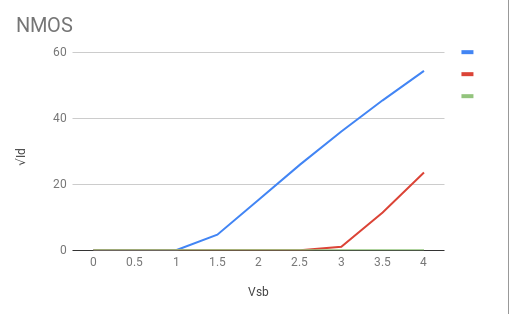
\includegraphics[width=4 in]{nmos_vt.png}
		\caption{NMOS \(\sqrt{I_D}\) vs. \(V_{DS}\)}
		\label{fig:nmos_vt}
	\end{figure}

	\begin{table}[H]
		\centering
		\caption{NMOS \(I_D\) vs. \(V_{DS}\) data}
		\label{table:nmos_vt}
		\begin{tabular}{|r||c|c|c|}
			\hline
			{\(\mathbf{V_{DS}}\) (\si\volt)} & \multicolumn{3}{|c|}{\(\mathbf{I_D}\) (\si{\micro\ampere})}\\
			\hline
			\(V_{SB}\) & 0\si{\volt} & 2\si{\volt} & 5\si{\volt}\\
			\hline
			0 & 0 & 0 & 0\\
			0.5 & 0 & 0 & 0\\
			1 & 0 & 0 & 0\\
			1.5 & 22.2 & 0 & 0\\
			2 & 234.1 & 0 & 0\\
			2.5 & 673.2 & 0 & 0\\
			3 & 1294.4 & 1.2 & 0\\
			3.5 & 2062.8 & 131.3 & 0\\
			4 & 2950.5 & 555.9 & 0\\
			\hline
		\end{tabular}
	\end{table}

	\begin{figure}[H]
		\centering
		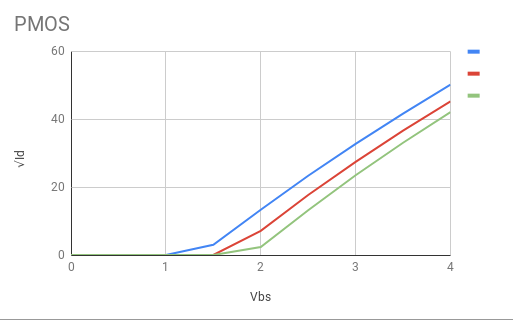
\includegraphics[width=4 in]{pmos_vt.png}
		\caption{PMOS \(\sqrt{I_D}\) vs. \(V_{DS}\)}
		\label{fig:pmos_vt}
	\end{figure}

	\begin{table}[H]
		\centering
		\caption{PMOS \(I_D\) vs. \(V_{SD}\) data}
		\label{table:pmos_vt}
		\begin{tabular}{|r||c|c|c|}
			\hline
			{\(\mathbf{V_{SD}}\) (\si\volt)} & \multicolumn{3}{|c|}{\(\mathbf{I_D}\) (\si{\micro\ampere})}\\
			\hline
			\(V_{BS}\) & 0\si{\volt} & 2\si{\volt} & 5\si{\volt}\\
			\hline
			0 & 0 & 0 & 0\\
			0.5 & 0 & 0 & 0\\
			1 & 0 & 0 & 0\\
			1.5 & 9.1 & 0 & 0\\
			2 & 177.9 & 50.6 & 5.5\\
			2.5 & 546.8 & 313.4 & 174.7\\
			3 & 1076 & 756 & 553.6\\
			3.5 & 1741.4 & 1346 & 1097.2\\
			4 & 2525 & 2053 & 1780.1\\
			\hline
		\end{tabular}
	\end{table}
	
	It's important to note, during the experiment, none of the given values of 
	\(V_{SD}\) for \(V_{SB} = 5 \si\volt\) were enough to cause the NMOS transitor to turn on. In order to 
	get some meaningful data out of that dataset, the minimum voltage that was
	required to turn on the MOSFET was recorded as 4.8 \si\volt. 

	\hfill \break

	A linear regression was used to find a line of best fit for the extraction
	of the transconductance parameter (\(k\)) and the threshold voltage (\(V_t\)).
	The experimental values for \(V_t\) that were found can be seen in Table
	\ref{table:experimental_vt} and the experimental value for \(k\) can
	be seen in Table \ref{table:experimental_body}.

	\begin{table}[H]
		\centering
		\caption{MOSFET \(V_t\) parameter extraction}
		\label{table:experimental_vt}
		\begin{tabular}{|c|c|c|}
			\hline
			\(\mathbf{|V_{SB}|}\) (\si\volt) & \multicolumn{2}{|c|}{\(\mathbf{V_t}\) (\si\volt)}\\
			\hline
			& NMOS & PMOS\\
			\hline
			0 & 1.23 & 1.30\\
			2 & 2.96 & 1.59\\
			5 & 4.8 & 1.85\\
			\hline
		\end{tabular}
	\end{table}

	\begin{table}[H]
		\centering
		\caption{MOSFET \(k\) parameter extraction}
		\label{table:experimental_body}
		\begin{tabular}{|c|c|c|}
			\hline
			\textbf{MOSFET} & \(\mathbf{k}\) & \(\mu\)\\
			\hline
			NMOS & 21.1959 & 2.1196 \(\times 10^{7}\)\\
			PMOS & 19.2986 & 1.9297 \(\times 10^{7}\)\\
			\hline
		\end{tabular}
	\end{table}
	
	A graph of \(V_t\) vs. \(\sqrt{2\phi_f + |V_{SB}|} - \sqrt{2\phi_f}\) was
	created in order to extract the body-effect parameter (\(\gamma\)) for both
	the NMOS and PMOS transistors. This graph and the value for \(\gamma\) can 
	be seen in Figure \ref{fig:body-effect} and Table \ref{table:body-effect}.

	\begin{figure}[H]
		\centering
		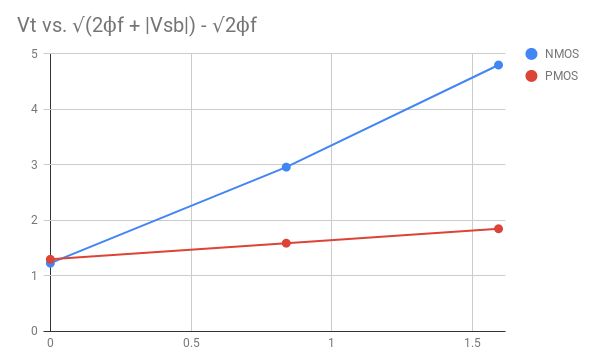
\includegraphics[width=4 in]{vt_vsb_body.png}
		\caption{\(V_t\) vs. \(\sqrt{2\phi_f + |V_{SB}|} - \sqrt{2\phi_f}\)}
		\label{fig:body-effect}
	\end{figure}

	\begin{table}[H]
		\centering
		\caption{Body-effect Parameter (\(\gamma\))}
		\label{table:body-effect}
		\begin{tabular}{|c|c|}
			\hline
			\textbf{MOSFET Type} & \(\gamma\)\\
			\hline
			NMOS & 2.24\\
			PMOS & 0.346\\
			\hline
		\end{tabular}
	\end{table}
	
	The next step in the experiment was to find the substrate doping parameter
	\(N_{sub}\) using two different methods. The first uses Equation
	\ref{equ:body-effect} and the second uses Equation \ref{equ:n_sub_2}.
	
	\begin{equation}
		\label{equ:n_sub_2}
		\mu = \mu_{min} + \frac{\mu_{max} - \mu_{min}}{1+(\frac{N_{sub}}{N_{ref}})}
	\end{equation}

	Rearranging Equation \ref{equ:body-effect} for \(N_{sub}\), a simple
	equation is derrived (\ref{equ:n_sub_1}).

	\begin{equation}
		\label{equ:n_sub_1}
		N_{sub} = \frac{(\gamma C_{ox})^2}{2q\varepsilon_s}
	\end{equation}

	Using the extracted value of \(\gamma\) and the assumed values for \(C_{ox}\)
	, \(q\), and \(\varepsilon_s\), the value for \(\gamma\) can be calculated.
	This value can be found in Table \ref{table:Nsub}.
	
	\hfill \break

	Rearranging Equation \ref{equ:n_sub_2} for \(N_{sub}\), a slightly
	more complex equation is derrived (\ref{equ:n_sub_2d}).

	\begin{equation}
		\label{equ:n_sub_2d}
		N_{sub} = N_{ref}\bigg(\frac{\mu_{max} - \mu_{min}}{\mu-\mu_{min}} - 1\bigg)
	\end{equation}
	
	Using the given values for \(\mu_{max}\), \(\mu_{min}\), \(N_{ref}\) and the 
	experimental values for \(\mu\), the \(N_{sub}\) parameter can be calculated.
	This value can also be found in Table \ref{table:Nsub}.
	\begin{table}[H]
		\centering
		\caption{Calculated \(N_{sub}\) values}
		\label{table:Nsub}
		\begin{tabular}{|c|c|c|}
			\hline
			\textbf{MOSFET Type} & \(\mathbf{N_{sub}}\) (Method 1) & \(\mathbf{N_{sub}}\) (Method 2)\\
			\hline
			NMOS & 134.017 & 9.2$\times 10^{13}$\\
			PMOS & 3.19754 & 2.23$\times 10^{14}$\\
			\hline
		\end{tabular}
	\end{table}

	These two methods for finding $N_{sub}$ produced vastly different values.
	this is partly due to the fact that one method assumes uniform substrate
	doping, which is not the reality. Also, the large difference between the
	values could be due to calculation errors. This seems like the most likley
	reason due the the extremly large difference between the values.

	\hfill \break

	The last part of the exercise was to extract the channel length modulation
	parameter ($\lambda_p and \lambda_n$). This was done by plotting $I_D$ vs.
	$|V_{DS}|$ and using a linear regression to fit the curve created when the
	device is in saturation. The x-intercept of this line is the early voltage
	($V_A$). The $\lambda$ is then the inverse of the early voltage. Figure
	\ref{fig:nmos_id_vs_vds} and \ref{fig:pmos_id_vs_vds} shows the graph of
	$I_D$ vs. $|V_{DS}|$ for both the NMOS and PMOS devices.

	\begin{figure}[H]
		\centering
		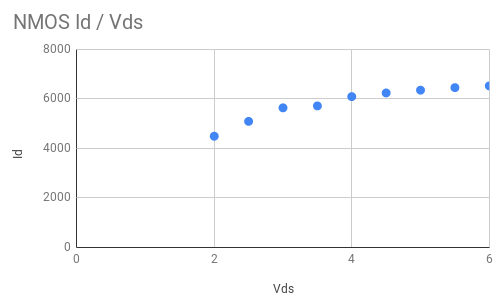
\includegraphics[width=4 in]{nmos_id_vds.png}
		\caption{NMOS $I_D$ vs. $|V_{DS}|$}
		\label{fig:nmos_id_vs_vds}
	\end{figure}

	\begin{figure}[H]
		\centering
		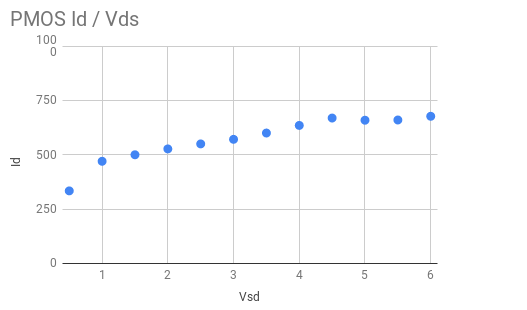
\includegraphics[width=4 in]{pmos_id_vds.png}
		\caption{PMOS $I_D$ vs. $|V_{DS}|$}
		\label{fig:pmos_id_vs_vds}
	\end{figure}

	The $|V_A|$ values that were found using the trendline when the device
	was in saturation can be found in Table \ref{table:early_voltage}.

	\begin{table}[H]
		\centering
		\caption{Extracted $|V_A|$ and $\lambda$}
		\label{table:early_voltage}
		\begin{tabular}{|c|c|c|}
			\hline
			\textbf{MOSFET Type} & \(|\mathbf{V_A}|\) & $\lambda$\\
			\hline
			NMOS & 56.6 & 0.01767\\
			PMOS & 19.7 & 0.05076\\
			\hline
		\end{tabular}
	\end{table}

	These values were relativley close for the values of $V_A$ found on the
	datasheet for the NMOS and PMOS transistors. 

	\section{Conclusion}
	The goal of this lab was to understand the different parameters in
	DC and AC biasing of MOSFET transistors. Parameters such as $k$, $V_t$,
	$\mu$, $\gamma$, and $\lambda$ were extracted using graphs and relationships
	between $I_D$ and $V_{DS}$. Most of the experimentally found values agreed
	with the theorized values, except for the second method for finding
	$N_{sub}$.
\end{document}
